%%%%%%%%%%%%%%%%%%%%%%
\chapter*{Checklist} %
%%%%%%%%%%%%%%%%%%%%%%
%\thispagestyle{empty}
Before going into a detailed discussion of how a paper/report should look like, we want to give a summary of the most important aspects. 
They should be checked before submitting any document, no matter whether it is for receiving feedback or as a final submission! 

\begin{itemize}
  \renewcommand\labelitemi{\Large$\Box$} % for checklist-alike appearance
  \item Required Information: Name, enrollment number, affiliation according to TUM requirements
   \begin{itemize}
     \item[$\triangleright$] Chair of High-Frequency Engineering, Department of Electrical and 
                             Computer Engineering, Technical University of Munich
     \item[$\triangleright$] \emph{Either} 80290 Munich, Germany 
                             \emph{or}     Arcisstraße 21, 80333 Munich, Germany
   \end{itemize}
  \item Minimum and maximum page limits
  \item All template content removed from final document
  \item Bibliography: All references in same style and including all information
  \item Present tense (past tense only for conclusions)
  \item Correct grammar: Articles, complete sentences (subject---predicate---object)
  \item Logical line of arguments without gaps
  \item Non-original content (above all, pictures and equations!) referenced
  \item Text in pictures is readable, best if fonts match
  \item Pictures should be readable if printed black-and-white/gray-scale only
  \item Every picture referenced before their first appearance or on same page
  \item Equations referenced only after their first appearance
  \item All variables and acronyms introduced at first appearance
  \item Equations embedded into text flow
  \item \emph{Variables italic}, mathematical constants upright, subscripts upright
  \item Consistent and invariable use of same symbols for same variables
\end{itemize}

\pagebreak % checklist on own page

%%%%%%%%%%%%%%%%%%%%%%%%%%%%%%%%%%%%%%%%%%%%%%%%
\chapter{The Imperative of Scientific Writing} %
%%%%%%%%%%%%%%%%%%%%%%%%%%%%%%%%%%%%%%%%%%%%%%%%
A scientific paper or report is written in order to publish new (scientific) results. 
Thus, it should make \emph{clear} what the new scientific results are.
Alas, scientific writing is not a discipline taught in school and it is, if at all, only taught rudimentarily at university.
The general expectation is that a student learns scientific writing by osmosis:
the student is supposed to acquire the writing skills for a successful career in academia by absorbing the style used in the respective scientific community.
Even if we would assume that the average writing style is good, ``learning by osmosis'' can hardly be called a ``target-oriented'' learning technique.

Most engineering students would typically never consider writing as their primal strength (typically backed by negative experiences with writing in high school): 
there seems to be a lack of any rules which would define what good scientific writing is, rules which could be used as measure to judge whether a sentence, a paragraph, a chapter, or even an entire document is good or not.

Fortunately, this is not true. 
In fact, when it comes to scientific writing there is only one imperative---\emph{clarity!}
Reading a paper with a difficult technical content is cumbersome simply because the material itself is difficult. 
If the material is presented in a form hard to understand and digest, maybe even so hard that it is not clear whether the material is difficult or only the writing so obstructive that the material seems to be difficult, a reader might simply decide not to further waste his time.
Remember: no one has to read your crap and those who have to read it (because they are examiners or reviewers) will not be grateful if they feel that the author actually does not care about the readers---why should they then care about the author?

Thus to keep your readership happy, the burden of reading your document should be relieved as much as possible. 
What makes reading a document burdensome is unclarity: 
obscure and long-winded sentences, wrong technical terms, wrong grammar, inconsistency in (mathematical) notation, logical gaps---in short, everything that forces a reader to spend his (precious) time on trying to understand what the author wanted to say.
The clearer a document is written, the more time the reader can spend on thinking about the actual content.

The good news, as has been pointed out by Ludwig Wittgenstein~\cite{wittgenstein_tractatus_1999}, is that ``what can be said at all can be said clearly, and what we cannot talk about we must pass over in silence.'' 
The purpose of this document is to show you how you can make \emph{clarity} the polar star of your writing. 
Given that an abundance of books have been written on this subject, any effort in this direction must remain fragmentary.
What can be done here is to lay the foundation and to sensitize you to typical obstacles in writing.
We will, however, refer to books that discuss the respective aspect in greater detail. 

We distinguish two main aspects: the style of writing and the structure of the document. 
In the style of writing section, we consider concepts that help to make a sentence (or paragraph, chapter etc.)
easier to grasp---concepts that will not, however, provide a single solution strategy and thus no black-and-white answer---and we discuss rules that are indeed black-and-white; 
for example, rules concerning the spelling or punctuation. 
In the structure of a document section, we explain that there are certain structural elements that every document in scientific writing should contain, such as the introduction,  what purposes these elements have, and how they have to be written in order to provide clarity.
\clearpage

%%%%%%%%%%%%%%%%%%%%%%%%%%%%%%%%
\chapter{Grammar and Spelling} %
%%%%%%%%%%%%%%%%%%%%%%%%%%%%%%%%

For German language speakers, the situation is simple: 
if you do not know how a word is spelled, you look it up in the Duden. 
You are uncertain about a grammatical construction? Look it up in the Duden! 
In the English language, there is no such consensus. 
Most likely you are familiar with the distinction in British English and American English. Still, there is no Duden of ``British English'' available---at least not a single Duden.  
In fact, there are many ``Dudens'' available. 
They are referred to as style guides, and every journal, newspaper, or publisher can require his authors to stick one of these style guides. 

At our chair, the most important publishers are IEEE and Elsevier. 
The latter only requires one to stick to either American or British English, whereas the IEEE has an style guide of its own~\cite{IEEEStyle}. 
This style guide does not consider all scenarios and therefore states that the final authority for grammar is the ``Chicago Manual of Style''~\cite{_chicago_2017} and for spelling is the ``Webster’s New Collegiate Dictionary''~\cite{merriam-websterinc_merriam_2014}.
Given that the ``Chicago Manual of Style'' is a popular style guide, we recommend to stick its rules as long as there are not contradicting rules of your publisher. 
For the rare case that you cannot find a rule or recommendation in the ``Chicago Manual of Style,'' the most important principle is \emph{consistency}: 
if you are inconsistent in your choices, the reader will wonder whether there is a reason for your inconsistency. 
Bad luck for you if they\footnote{This is an example of the so-called ``singular they''. See \cite{_chicago_2017} for a discussion on this matter.} come to the conclusion that there is no reason except of laziness and  incompetence.

Without claiming any completeness, some of the most popular mistakes in grammar are:
\begin{itemize}
    \item The definite article “the” (singular and plural) is used to refer to a particular member of a group or class. 
    It may be something already mentioned or something uniquely specified.
    \item The indefinite articles “a/an” are only for singular use; 
    they indicate that their noun is not a particular, identifiable one. 
    \item Use of a/an: \emph{An} is used before words that begin with a vowel sound. 
    This is connected to phonetics and not to the following letter:
    \begin{itemize}\vspace*{-0.1cm}
        \item A user, a union, a one-year-old child, a team, a map.
        \item But an hour, an FFT, an onion, an elephant and an exit.
    \end{itemize}
    \item Adverbs and adpositional phrases at the beginning of a sentences are 
    separated by a comma: “However, \ldots”,  “Thus, \ldots” or “In the beginning, \ldots”
    \item Contractions such as “don’t” and “can’t” are not used in technical text. 
    Change to “do not” and “cannot.”
    \item The paper should be written in complete sentences; that is,  all sentences
    contain a subject followed by a predicate, and optionally objects or adverbials.
\end{itemize}
\clearpage

%%%%%%%%%%%%%%%%%%%%%%
\chapter{Typography} %
%%%%%%%%%%%%%%%%%%%%%%
What is typopgraphy\index{typography}? According to Wikipedia, 
``Typography is the art and technique of arranging type to make written language legible, readable, and appealing when displayed. 
The arrangement of type involves selecting typefaces, point sizes, line lengths, line-spacing (leading), and letter-spacing (tracking), and adjusting the space between pairs of letters (kerning[1]). 
The term typography is also applied to the style, arrangement, and appearance of the letters, numbers, and symbols created by the process.'' 
Following typographical rules helps you to make your document clearer. 

Some of these rules or recommendations are discussed in style guides and are considered as part of ``grammar'' and here, we just summarize the most important ones. 


%%%%%%%%%%%%%%%%%%%%
\section{Fonts} %
%%%%%%%%%%%%%%%%%%%%
The chosen fonts\index{typography!fonts} (Times New Roman, Arial, etc.) and font shapes (italic, upright, bold, etc.) for variables, functions, numbers, units, etc. must be used \emph{consistently} throughout the whole paper. 
In particular, the variables and numbers and units have the same fonts everywhere: 
in the text, in equations, and in figures.
For the sake of readability, it is a good idea to chose a serif font---such as Times New Roman, Libertine, Garamond, Minion---for the body text in an upright shape (not italic). 
Sans serif (Grotesque) fonts, such as Arial\index{Arial|see{typography}}, Helvetica, Myriad---may be used for title and headings. 
Though very commonly used, they are not suited for body text. 


%%%%%%%%%%%%%%%%%%%%%%
\section{Figures}    %
%%%%%%%%%%%%%%%%%%%%%%
Figures\index{typography!figures} are included into the flowing text and get a numbered figure caption. 
Every figure is referenced and discussed within the text, of course in an identical manner throughout the text: ``[\dots] as
shown in Fig.~7 and [\dots].''
All figures (and tables) must have a caption describing the content shown in the figure.
The first word of the caption text starts with a capital letter and the caption text ends with a period.
The IEEE style guide recommends to avoid using ``A,'' ``An,'' or ``The'' at the beginning of a caption~\cite{IEEEStyle}.   
A figure is placed in the text after it was referenced in the text, never before.
Variables, numbers, units, etc. in figures have the same style and fonts as everywhere else in the text. 
All figures are drawn in a way that they are still readable if printed in gray-scale. 
This also holds for colormaps.
Gray-scale readability can be realized by different means. 
Some of them are given in Figs.~\ref{fig:samplefigure} to~\ref{fig:samplefigure3}. %
\begin{figure}[tp]
    \centering
    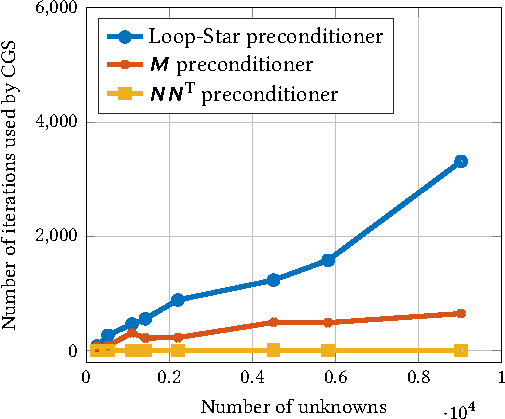
\includegraphics{./Figures/Fig_1__Results/Fig_1__Results.pdf}
    \caption{The caption should provide the essential information to distinguish this figure from other figures. 
        Note that the black-and-white discriminability is ensured by different marks for the data points.}
    \label{fig:samplefigure}
\end{figure}%	

\begin{figure}[tp]
    \centering
    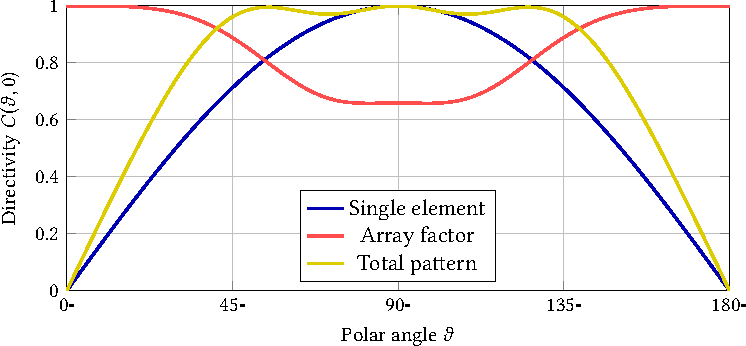
\includegraphics{./Figures/Fig_2__Array_radchar/Fig_2__Array_radchar.pdf}
    \caption{The caption should provide the essential information to distinguish this figure from other figures. 
        Note that the black-and-white discriminability is ensured by different gray-scale values of the curves in the plots.}
    \label{fig:samplefigure2}
\end{figure}%

\begin{figure}[tp]
    \centering
    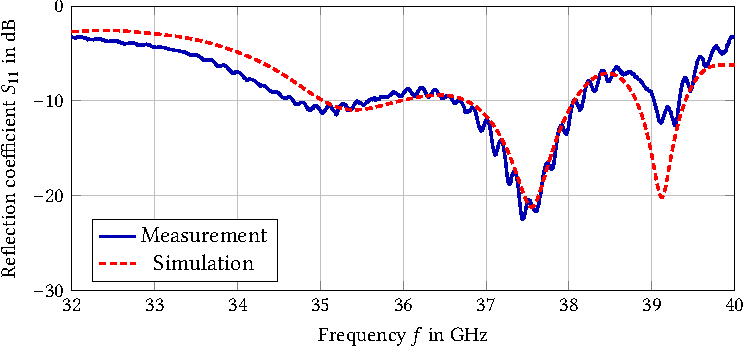
\includegraphics{./Figures/Fig_3__measure_dB/Fig_3__measure_dB.pdf}
    \caption{The caption should provide the essential information to distinguish this figure from other figures. 
        Note that the black-and-white discriminability is ensured by different line styles.}
    \label{fig:samplefigure3}
\end{figure}%

All figure axes have to be labeled with the quantity they represent and their according dimension/unit. 
The font and font size of the figure axis labels and axis tick labels should match to the caption. 
It is better to use words rather than symbols, e.g.\ “Frequency” or “Frequency $f$” instead of “$f$.”
It is \emph{wrong} to put the unit in square or any other kind of brackets, even though it is seen sometimes:
\begin{quote}\small
    Frequency $f$ [Hz] \hspace {1cm}\textbf{wrong!}
\end{quote}
The square brackets are an operator giving the unit of the quantity they act on, i.e.\ $[f]=\si{Hz}$. 
Therefore, we recommend to stick to DIN~461 (international versions: ISO~31-0 and~ISO 80000-1) and use either a division
\begin{quote}\small
    Frequency $f$ / Hz
\end{quote}
or the word “in”
\begin{quote}\small
    Frequency $f$ in Hz.
\end{quote}
In our opinion, the only possible exception are angles given in degree, since “in $^\circ$” or “/ $^\circ$” looks ugly. 
As an alternative to
\begin{quote}\small
    Azimuthal angle $\varphi$ in degree,
\end{quote}
one can also write the degree sign at each axis tick label, see Fig.~\ref{fig:samplefigure2}. 
Avoid writing units at each tick label for other units than degree, however.

The easiest way to achieve consistent labels in figures is to generate vector drawings during the \LaTeX\ compilation process. 
For drawings and plots, we recommend to use Ti\emph{k}Z or \emph{pgfplots}. 
If data is already present in MATLAB, one can use \emph{matlab2tikz}. 
Similarly, Julia offers packages to create Ti\emph{k}Z figures. 
An example for a figure created with Ti\emph{k}Z is Fig.~\ref{fig:samplefigure}. 
The alternative is to plot the data with \emph{pgfplots}. 
The settings regarding axes, linestyles, etc. are similar to the MATLAB options. 
Some example plots are shown Fig.~\ref{fig:samplefigure2}, Fig.~\ref{fig:samplefigure3} and Fig.~\ref{fig:samplefigure4}. 

Figures are commonly placed on the top of a page or on a single page for floating elements (options for \emph{figure} environment: \verb|[tp]|), less often on the bottom (\verb|[b]|) and never in the middle of a page (happens with \verb|[h]|). 
Do not use these commands while you are in the writing process. 
Use these options only for the final typesetting of the thesis and if necessary. 
\LaTeX~knows well where to place figures and tables best, but it cannot optimize their placement if you have used these options too often.

\begin{figure}[tp]
    \centering
    \begin{minipage}[b]{.5\linewidth}
        \centering
        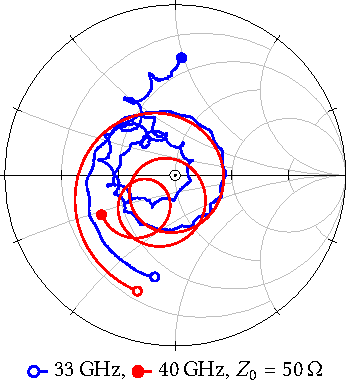
\includegraphics{./Figures/Fig_4__measure_smithchart/Fig_4__measure_smithchart.pdf}
        \subcaption{\mbox{}}\label{fig:1a}% place a subcaption here. Usually not done.
    \end{minipage}%
    \begin{subfigure}[b]{.5\linewidth}
        \centering
        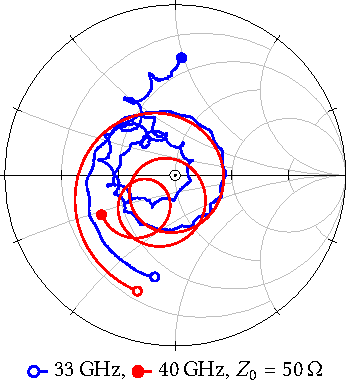
\includegraphics{./Figures/Fig_4__measure_smithchart/Fig_4__measure_smithchart.pdf}
        \caption{}\label{fig:1b}
    \end{subfigure}
    \caption{The caption should provide the essential information to distinguish this figure from other figures. 
        We use the \emph{subcaption} package for subfigures. 
        (a)~A subfigure on the left, created with the \emph{minipage} environment and the \emph{subcaption} macro. 
        (b)~Another subfigure on the right, created with  the \emph{subfigure} environment and the \emph{caption} macro. }
    \label{fig:samplefigure4}
\end{figure}		

A visualization of a Raw-Wilton-Glisson (RWG) basis function is shown in Fig.~\ref{label}.
\begin{figure}[tp]
	\centering
	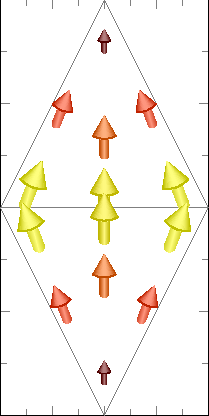
\includegraphics{./Figures/Fig_5__RWG/Fig_5__RWG.pdf}
	\caption{The caption should provide the essential information to distinguish this figure from other figures. 
		Note that the black-and-white discriminability is ensured by different line styles.}
	\label{fig:samplefigure3}
\end{figure}%


%% Test if gnuplot exists
%\newread\teststream
%\newcommand*\testline{}
%\openin\teststream={|gnuplot -V}
%\ifeof\teststream
%\typeout{Unable to open test stream.}
%\else
%\typeout{Test stream opened.}
%\read\teststream to \testline
%\typeout{\testline}
%\fi
%
%\StrLeft{\testline}{7}[\firstletters]%
%
%\ifthenelse{\equal{\firstletters}{gnuplot}}
%{
%    \Cref{fig:samplefigure6} is a combined surface/contour plot, which requires gnuplot for compilation.
%    \begin{figure}[tp]
%        \centering
%        %%%%%%%%%%%%%%%%%%%%%%%%%%%%%%%%%%%%%%%%%%%%%%%
%%%%%%%%%%%%%%%%%%%%%%%%%%%%%%%%%%%%%%%%%%%%%%%
%%%%%%%%%%%%%%%%%%%%%%%%%%%%%%%%%%%%%%%%%%%%%%%
% Definitions
%%%%%%%%%%%%%%%%%%%%%%%%%%%%%%%%%%%%%%%%%%%%%%%
%%%%%%%%%%%%%%%%%%%%%%%%%%%%%%%%%%%%%%%%%%%%%%%
%%%%%%%%%%%%%%%%%%%%%%%%%%%%%%%%%%%%%%%%%%%%%%%

\def\thispath{Plots/surf}

\usepgfplotslibrary{units}
\usepgfplotslibrary{colormaps}
\usetikzlibrary{pgfplots.colorbrewer}
\pgfplotsset{surf shading/precision=pdf}



\def\colorbartextwidth{1.75em}
\def\colorbarwidth{0.25cm}
\def\axislabelshift{0.125cm}


\pgfplotsset{
  colormap/hotsteep/.style={
colormap={hotsteep}{[1cm]rgb255(0cm)=(255,255,255) rgb255(27cm)=(255,255,254) rgb255(28cm)=(1,0,0)
rgb255(42cm)=(0,0,0)}
}}



%%%%%%%%%%%%%%%%%%%%%%%%%%%%%%%%%%%%%%%%%%%%%%%
%%%%%%%%%%%%%%%%%%%%%%%%%%%%%%%%%%%%%%%%%%%%%%%
%%%%%%%%%%%%%%%%%%%%%%%%%%%%%%%%%%%%%%%%%%%%%%%
% Plots (1 surf & 2 contour)
%%%%%%%%%%%%%%%%%%%%%%%%%%%%%%%%%%%%%%%%%%%%%%%
%%%%%%%%%%%%%%%%%%%%%%%%%%%%%%%%%%%%%%%%%%%%%%%
%%%%%%%%%%%%%%%%%%%%%%%%%%%%%%%%%%%%%%%%%%%%%%%

\begin{tikzpicture}

\begin{axis}[
             width = {0.6\linewidth-\colorbartextwidth-\colorbarwidth+\axislabelshift-0.05cm},
             ymin=-75,
             ymax=-15,
             ytick={-70,-60,-50,-40,-30,-20},
             grid=major, 
             axis on top,
             colorbar,
             colormap/viridis, 
             mesh/ordering=x varies,
             view={0}{90},
             colorbar style={
                             scaled ticks=false,
                             ytick={-150,-125,...,0},
                             width=\colorbarwidth,
                             yticklabel style={
                                               align=right,
                                               text width = \colorbartextwidth,
                                               },    
                             xlabel = {$P_\mathrm{IF} /\textrm{\si{dBm}}$},   
                             xlabel style = {xshift = 0.1875cm, yshift = {-0.51 cm +\axislabelshift},font=\small},  
                             xshift = -0.3cm,  
                             },
             xlabel style = {yshift = \axislabelshift},   
             ylabel style = {yshift = -\axislabelshift},    
             tick label style={/pgf/number format/fixed},
             enlargelimits=false,
             xlabel={$v_\mathrm D \textrm{ in \si{\volt}}$}, 
             ylabel={$P_\mathrm{RF} \textrm{ in \si{dBm}}$}, 
             ]
      \pgfplotstableset{skip first n = 1,}
      \pgfplotstableread{\thispath/power_bias.txt}\datatable
      
            \addplot3[
                     mesh/rows=13, 
                     surf,  
                     shader = interp,       
                    ] table [
                             x index = 1,
                             y  index= 0,
                             z index = 2,
                            ]   from \datatable {};
                            
\pgfplotsset{filter discard warning=false,
                        contour/every contour label/.style = {
                          sloped,
                          transform shape,
                           every node/.style={
                                              mapped color!90!white,
                                              fill=none,
                                              text opacity=0,
                                              },
                        },
}
            \addplot3[
                     mesh/rows=13, 
                     mesh/cols=31, 
                     thin,
                     colormap/hotsteep,
                     contour gnuplot={
                        levels={-100,-80,-60,-40,-30,-20},
                     },
                     contour/label distance=5500pt,
                    ] table [
                             x index = 1,
                             y  index= 0,
                             z index  = 2,
                            ]   from \datatable {};
                            
              
                            
                            
\begin{scope}
\clip
(axis cs:0.55,-75) -- (axis cs:0.55,-15) -- (axis cs:0.7,-15) -- (axis cs:0.7,-75) -- cycle;
                            
\pgfplotsset{filter discard warning=false,
                        contour/every contour label/.style = {
                          sloped,
                          transform shape,
                           every node/.style={
                                              mapped color!90!white,
                                              fill=none,
                                              text opacity=1,
                                              draw opacity=0,
                                              },
                        },
}
            \addplot3[
                     mesh/rows=13, 
                     thin,
                     mesh/cols=31, 
                     colormap/hotsteep,
                     %colormap/PuBu-9,
                     contour gnuplot={
                        levels={-100,-80,-60,-40,-30,-20},
                        contour label style={nodes={text=mapped color, text opacity=1,},font=\footnotesize},
                     },
                     contour/label distance=120pt,
                     contour/labels over line,
                     samples=200,
                     %={
                     % number=24,
                     % % cdata should not be affected by z filter:
                     % output point meta=rawz,
                     % labels=false,
                     %},
                     %point meta = explicit,
                    ] table [
                             x index = 1,
                             y  index= 0,
                             z  index = 2,
                             %meta expr = -\thisrowno{2},
                            ]   from \datatable {};
\end{scope}                            
        %
            
\end{axis}
\end{tikzpicture}
%        \caption{The caption should provide the essential information to distinguish this figure from other figures.}
%        \label{fig:samplefigure6}
%    \end{figure}
%}{
%    \Cref{fig:samplefigure6} is commented out, since it requires gnuplot for compilation.
%}


\section{Tables}
Everything said for figures is also true for tables, where tables are however numbered independently: 
As seen in Tab.~7, \dots

Avoid vertical lines. 
Avoid double lines. Use \verb|\toprule|, \verb|\midrule| and \verb|\bottomrule| for horizontal lines.
Avoid ``boxing up'' cells. If there is enough space between the content, the alignment of the text is sufficient to create column separation as in Tab.~\ref{tab:tabellensatz}. 
The usage of midrules for a better overview can bee seen in Tab.~\ref{tab:linien}. 


A higher degree of hirarchy can easily be created by using midrules and multicoloumns as in Tab.~\ref{tab:sampletable}. 
If in doubt, align the cell content on the left. 
However long numbers with varying number of digits may be aligned on the right for a better overview.

Do not confuse a table and a tableau. 
A table is organized in columns, while a tableau organizes information in matrix form. 
% For a tableau, vertical lines are ok. 

In Tables, the \texttt{S} column type should be used for numbers as illustrated in \Cref{tab:sampletable}. 
The \texttt{S} column type is part of the \emph{siunitx} package and provides a proper alignment of the numbers.
\footnote{Footnotes are not common in an engineering thesis, but they can definitely be used.}


\begin{table}[tp]
    \centering
    \caption{Avoid vertical lines}
    \label{tab:tabellensatz}
    \begin{tabular}{@{}*{4}{l}@{}}
        \toprule
        Nominativ & Genetiv & Dativ & Akkusativ \\
        \midrule
        die Frau & der Frau   & der Frau  & die Frau \\
        der Mann & des Mannes & dem Manne & den Mann \\
        das Kind & des Kindes & dem Kinde & das Kind \\
        \bottomrule
    \end{tabular}
\end{table}%
%
\begin{table}[tp]
    \centering
    \caption{Usage of lines}
    \label{tab:linien}
    \begin{tabular}{@{}l*{4}{c}@{}}
        \toprule
        Month & 1965 & 1966 & 1967 & 1968 \\
        \cmidrule(r){1-1}\cmidrule(lr){2-2}\cmidrule(lr){3-3}\cmidrule(lr){4-4}%
        \cmidrule(l){5-5}
        September & 2000 & 1700 & 2300 & 1900 \\
        October   & 1500 & 1800 & 1900 & 3000 \\
        November  & 2500 & 2800 & 4700 & 3200 \\
        December  & 2300 & 2000 & 3600 & 2700 \\
        \bottomrule
    \end{tabular}
\end{table}	  

\begin{table}[tp]
    \centering
    \caption{Memory and time consumption for the double layer and adjoint double layer discretizations.}
    \label{tab:sampletable}
    \begin{tabular}{@{}*{2}{l}*{4}{S}@{}}
        \toprule 
        \multicolumn{2}{N}{Function} &
        \multicolumn{1}{N}{CPU} &			
        \multicolumn{1}{N}{Memory} &
        \multicolumn{2}{N}{Time} 
        \\
        \cmidrule(r){1-2}
        \cmidrule(l){5-6}
        \multicolumn{1}{N}{Source} &  
        \multicolumn{1}{N}{Test} &	
        &  
        &  			
        \multicolumn{1}{N}{CG} &
        \multicolumn{1}{N}{Total} 
        \\
        & & \multicolumn{1}{N}{$\#$}&  \multicolumn{1}{N}{in GB}&  \multicolumn{1}{N}{in s} & \multicolumn{1}{N}{in s}
        \\
        \cmidrule(r){1-1} \cmidrule(lr){2-2} \cmidrule(lr){3-3} \cmidrule(lr){4-4} \cmidrule(lr){5-5}  \cmidrule(l){6-6} 
        \multicolumn{5}{@{}L}{\emph{Adjoint Double Layer Discretizations}}  \\
        $p$ & $p$ & 54 & 642 & 350 & 19790 \\
        $p$ & $\hat{\lambda}$ & 54 & 642 & 408 & 25786 \\
        $\lambda$ & $\lambda$ & 54 & 160 & 103 & 37672 \\
        \multicolumn{5}{@{}L}{\emph{Double Layer Discretizations}}  \\
        $p$ & $p$ & 54 & 642 & 340 & 18486 \\
        $\lambda$ & $\hat{p}$ & 54 & 160 & 120 & 24210 \\
        $\lambda$ & $\lambda$ & 54 & 160 & 100 & 35321 \\
        \bottomrule \addlinespace
    \end{tabular}
\end{table}


%%%%%%%%%%%%%%%%%%%%%%%%%%%%%%%%%%%%%%%%%%%%%%%%%%%%%%%%%%
\section{Micro Typography and Related \LaTeX\ Macros} %
%%%%%%%%%%%%%%%%%%%%%%%%%%%%%%%%%%%%%%%%%%%%%%%%%%%%%%%%%%
In German texts, abbreviations have half spaces between the single letters. 
Do not use ``z.B.'' (\emph{wrong}!) but ``z.\,B.'' (correct!). 
A half space can be introduced with the \LaTeX -command \verb|\,| (backslash followed by comma). 
In English, however, it is the other way around. Correct is ``i.e.'' but not ``i.\,e.''. 
To ensure correct spacing after a period, it is important to write “i.e.\verb|\|\Vtextvisiblespace[.5em]~,” i.e., the abbreviation period is followed by a backslash and a blank to ensure correct spacing. 
The spacing after a sentence-ending period is commonly a bit larger than the normal inter-word spacing. 

The \emph{hyphen} ``-'' is used to combine several words into a single entity like in ``finite-element-method''. 
This is mainly done for the combination of at least three words, to indicate the stronger binding of the first words: 
3-dB bandwidth or combined-source condition.

If one wants to express an interval from $A$ to $B$, one can use the \emph{en dash} ``--'' generated by the command \verb|--| or the UTF-8 symbol \verb|–|: $A$--$B$ without any space or $A$\,--\,$B$ with a half space.

It is different from the \emph{em dash} ``---,'' which is used for a break in a sentence or to set off parenthetical statements---like this statement---, while punctuation is not separated by a blank from the dash. 
An em dash is significantly longer than a hyphen and even longer than the en dash. 
It is generated via \verb|---|.  

Another completely different symbol is the minus sign “$-$”. 
Since it does never occur in normal text, but only in a mathematical context, it is generated in math mode as \verb|$-$| and automatically when the  \verb|\SI| command is used.

For quotation marks, use “\ldots” for American English texts and ‘…’ for British English texts.  
They can be generated by \verb|``|(starting the quote) and \verb|''|(ending the quote) or, more easily, by the UTF-8 symbols “…”.	 Nested quotation marks are indicated by  ‘…’ and “\ldots”, respectively. 
Notice, that there is no space between the quotation marks and the first or last letter of the quotation. 
Also, the quotation marks have to stick to the words at the beginning or the end of a line, i.e., they must not be separated by a line break from the first or last word of the quotation. 
In English text, the periods and commas are within the quotation marks:
\begin{quote}\small
    This is an example sentence “including a quote.”
\end{quote}
However, other punctuation appears “outside”!

For German texts use either \glqq\ldots\grqq\ (generated by \verb|\glqq| and \verb|\grqq|) or >>\ldots<< (generated by \verb|>>| and \verb|<<|).
Using the UTF-8 symbols „…“ and »…« is also possible. 
Nested quotation marks are denoted as ‚…‘ and ›…‹.
In German text, the punctuation happens outside the quotation:
\begin{quote}\small
    Ein Beispielsatz „enthält ein Zitat“.
\end{quote}

Whatever convention is chosen, has to be strictly kept throughout the whole text. 

The apostrophe is not a quotation mark, it is used for the s-genitive---the student's report---and written as \verb|'| in the source code. 
For typesetting minutes and seconds, we recommend the \emph{siunitx} package: 
\ang{;1;59} (\verb|\ang{;1;59}|) means one minute 59 seconds. 

Numbers with up to three numerals are not separated by spaces, e.g.\ \num{100}. 
For numbers consisting of more than four numerals, the numerals are grouped in groups of three and a space (thousands separator, dt.\ Tausendertrennzeichen) is introduced between the so grouped numerals, e.g.\ 10\,000; for numbers with four numerals, the thousands separator is optional. 
Alternatively, a comma is used, e.g.\ 1,000, while the period is used as decimal separator, e.g.\ \num{3.141}.
In German, it is the other way round: The decimal places are separated by a comma, e.g.\ 3,141, while a half space and a period can be used as thousands separator.
The command \verb|\num{3.141}| from the \emph{siunitx} package can help to typeset numbers correctly, according to the chosen language setting. 

A \emph{paragraph} helps to structure the text within a section or subsection. 
A paragraph can be produced by inserting a blank line between two lines of code in the tex-source (which is the preferred way since the readability of the document is increased) or by the TeX macro (\verb|\par|). 
A paragraph is not ended by the newline macro  (\verb|\newline|) and the macro \verb|\\|. 
Both just start a new line, while \verb|\\[1cm]| takes an optional argument for extra space and is generally preferred. 
% see http://texwelt.de/wissen/fragen/4014/was-ist-der-unterschied-zwischen-newline-und-linebreak
Another similar command is the line break (\verb|\linebreak|), which can help to fine tune the line breaks of some text. 
In contrast to \verb|\\|, it stretches the text of the broken line to its end. 
The line break macro has an optional penalty argument to define the urgency of the break. 
The \verb|\nolinebreak| macro indicates that no line break should ever happen at this place. 
The \verb|\allowlinebreak| macro gives the hint that a line break can happen at this place. 
In a similar way, \verb|\-| gives the hint that a line break with hyphenation might occur inside a word, e.g.\ \verb|Ar\-beiter\-unfalls\-ver\-si\-che\-rungs\-ge\-setz|. 
However, this should only be used for single occurances of a word. The better option is to maintain a list of complicated words with the hyphenation command: \verb|\hyphenation{Ar-beiter-unfalls-ver-si-che-rungs-ge-setz}|.

% http://texwelt.de/wissen/fragen/18/was-ist-der-unterschied-zwischen-newpage-pagebreak-und-clearpage
Quite simular commands exist for page breaks. 
The \verb|\newpage| macro ends a page (or column in two-column mode), leaves the remaining space white and continues on the top of a new page or column. 
The \verb|\clearpage| macro ends a page and places all open floating environments (figures, tables) on as many pages as needed. \verb|\cleardoublepage| does the same for two-sided documents. 
The \verb|\pagebreak| macro ends a page and stretches whitespaces to flush the text to the lower page border.  
The page break macro has an optional penalty argument to define the urgency of the break. 
The \verb|\nopagebreak| macro indicates that no page break should ever happen at this place. 

Highlighting/Emphasis in the text: 
Do \emph{never} use underlining, since it does not match to anything else in the text. 
Avoid \textbf{bold} text, because it is too much active emphasis and changes the type color (dt. Grauwert) of the text. 
Bold text can be used for headings, tables, etc.
The \verb|\emph| macro is preferred to generate italic text. 
In general, italic text is preferred  over oblique (slanted) text.

%%%%%%%%%%%%%%%%%%%%
\section{Lists} %
%%%%%%%%%%%%%%%%%%%%
A sample list:
\begin{enumerate}
    \item First item
    \item Second item
\end{enumerate}
Also, consider the \emph{enumitem} package for more sophisticated lists.

In scientific documents enumerations are rarely seen. 
If you feel that you have to use a list, please consult \cite{_chicago_2017} for the correction punctuation.
\clearpage


%%%%%%%%%%%%%%%%%%%%%%%%%%%%
\chapter{Style of Writing} %
%%%%%%%%%%%%%%%%%%%%%%%%%%%%
The language of a scientific paper or a report is also scientific and technical. 
A paper is not written as an adventure report. 
In particular, it is not appropriate to write about your feelings. 
Nevertheless, the main objective of any scientific text is to provide a \emph{clear} message. 
Thus, while the language shall be scientific and technical, use scientific and technical terms for good and utilize them in order to make your text more clear and do not use fancy terminology only to impress people.

Writing is editing.
Writers of a scientific or technical text is spend a large portion of their time with editing their text. 
Often they face the problem, that a passage of the text is hard to read and understand or just does not read ``fluently''.
Spotting the problem is one thing, but curing the illness is a completely different story. 
In this section, tools are presented to improve the readability of a text.
  
%%%%%%%%%%%%%%%%%%%%%%%%%%%%%%%%
{Action and Heroes} %
%%%%%%%%%%%%%%%%%%%%%%%%%%%%%%%%
The \emph{action and heroes} principle states that the subjects of the sentence should name the heroes
and the verbs that go with those subjects should name the crucial actions those heroes are part of.
 
Consider the following example:
\begin{quote}
	\small
	The cause of our educational system's failure at teaching basic skills to all children is not understanding the influence of their cultural background on learning.
\end{quote} 
Its content is identical to the following sentence:
\begin{quote}
	\small
	Our educational system has failed to teach all children	basic skills because we do not understand how their cultural background influences the way they learn.
\end{quote}
Most people have less difficulties to understand the content of the second example. 
The reason for this is that the grammatical structure of the second example correctly hints to what is happening (the \emph{action}) and who is performing the action (the \emph{hero}). 
Grammatically, the subject of the first sentence is ``{the cause of our educational systems failure}'' and the verb is ``to be'', while the subject of the second sentence is ``our educational system'' and the corresponding verb is ``has failed''. 
It is usually a good sign when a sentence can be stripped from everything except its subject and its verb and still makes sense. 
The action and heroes principle suggests to prefer active voice over passive voice and to avoid nominalizations.
%%%%%%%%%%%%%%%%%%%%%%%%%%%%%%%%%%%%%
\section{Cohesion and Coherence} %
%%%%%%%%%%%%%%%%%%%%%%%%%%%%%%%%%%%%%
While the \emph{actions and heroes} principle works locally on sentence level, \emph{cohesion and coherence} is about combining sentences in order to create a text that ``flows.''
\emph{Cohesion} is the glue that sticks together the individual sentences. 
Natural cohesion can be implemented by forming sentences which contain a part of old information and a part of new information. 
By starting a sentence picking up the new information from the previous sentence as an old information and letting the sentence end with a new information, a natural text flow is created as illustrated by the following example:
\begin{quote}
\small
Some astonishing questions about the nature of the universe have been raised by scientists exploring the nature of \emph{black holes} in space.  A \emph{black hole} is created by the collapse of a dead star into a point perhaps not larger than a \emph{marble}. So much \emph{matter compressed into so little volume} changes the fabric of space around it in profoundly puzzling ways.	
\end{quote} 
The portions of new and old information are emphasized in italics.

The passive voice can help to restructure the sentence, such that the old information appears at the beginning of the sentence.
This highlights the importance of not being dogmatic about stylistic rules, but to know and apply the appropriate tools, once a stylistic faux-pas has been spotted.

\emph{Coherence} names the principle of having a clear idea per paragraph. A paragraph should have a clear topic and a guiding \emph{thread}. When you start a paragraph about why roses are red, you should not end the paragraph with your food preferences for dinner.  
%%%%%%%%%%%%%%%%%%%%%%%%%%
\section{Weasel Words}%
%%%%%%%%%%%%%%%%%%%%%%%%%%
Weasel words are phrases or words that sound good without conveying information.
They obscure precision of a statement and should therefore be avoided.
They are named this way, because the weasel is known for sucking the content of raw bird eggs for food and leaving the empty hull behind.
This is, what weasel words will do with your sentences.

A typical variation of weasel words comes in the form of \emph{salt and pepper words}. 
These are words, which one strews over the sentences like spices over food. 
Typical salt and pepper words are \emph{various, a number, fairly,} or \emph{quite}.

Another common type of weasel words are \emph{beholder words}.
These are words which convey a personal opinion without naming the beholder.
Typical examples for beholder words are \emph{interestingly, surprisingly, remarkably},  or \emph{clearly}, as e.g. in the sentence ``False positives were surprisingly low''.
These words should also be avoided. 
If you want to express, that you were surprised, than make the beholder explicit, e.g. by ``To our surprise, false positives were low (\SI{3}{\percent} )''.

Finally, there are the \emph{lazy words}. 
These are words which are used to pretend to convey quantitative information, when the writer is actually to lazy to be quantitative.
Typical lazy words like \emph{very, extremely, several, exceedingly, many, most, few, vast, relatively, greatly, substantially, huge,} or \emph{tiny} should be avoided, when no further quantification is given.

%%%%%%%%%%%%%%%%%%%%%%%%%%%%%%%%%%%%%%%%%%%%%%%
\section{On the Usage of ``We'' and ``I''} %
%%%%%%%%%%%%%%%%%%%%%%%%%%%%%%%%%%%%%%%%%%%%%%%
%It is not written in the I form (i.e., “[\dots] and then I experienced  [\dots]”).
%Usually, passive form is a good choice for writing the paper:  
%``[\dots] in the following, several derivations and arguments are presented [\dots].''
%Some people use the we form: ``[\dots]  in the following, we present [\dots].''
%However, this might not be the right style for a master student or doctoral candidate.
The opinions on the usage of the personal pronouns ``we'' and ``I'' vary greatly. 
The classical advise is to avoid them entirely and use the passive voice if necessary to do so.
This is, in particular, true for the German language. 
Numberless examples exist for an inappropriate (i.e., not technical) use of the personal pronouns:
\begin{itemize}
    \item This task presented a big challenge for us. \qquad\textbf{wrong!}
    \item This task was very educational for us as it gave us knowledge and experience. \qquad\textbf{wrong!}
    \item As we believe, there might be multiple solutions. \quad\textbf{wrong!}
    \item First, we calculated $\omega=0.226$ and, next, we tried to find the right values for further calcuations. \qquad\textbf{wrong!}
\end{itemize}

Nevertheless, when it comes to mathematical writing in English language, we have to note that certain expressions require the usage of ``we''. 
For example, in German we often write ``es gilt, dass $a=b$'', which literally translates to ``it holds that $a=b$.''
This, however, is a Germanism. 
Instead the correct translation is rather ``we have that $a=b$'', or alternatively, ``[...] and $a=b$ holds.''
Thus, commonly used expressions in mathematical writing such as ``we have'', ``we find'',  or ``we obtain'' require the use of ``we'', which refers in this context ``the author(s) and the reader''.
This is---at least in the English language---a commonly used practice.

When you are author of a document with multiple authors, it is also commonly accepted to use ``we'' referring to ``the authors''. 
Usually, it should be clear from the context whether ``we'' refers only to the authors or to the authors and the reader. 
If it is not clear, one can use ``the authors'' instead of ``we''.
This should not be done excessively since it sounds a bit pompous.

For a thesis, however, you are the single author and using ``we'' to refer to yourself is odd, both in German and in English.
The classic strategy is to use the passive voice, a strategy though that leads less clarity:
\begin{quote}
    \small
    It was hypothesized that this is due to infrequent or short interactions between S. Typhimurium and Y. enterocolitica. To test these hypotheses, an S. Typhimurium strain that synthesizes AHLs to mimic a constant interaction with Y. enterocolitica was constructed. [Journal of Bacteriology (2010) 192.1: 29]
\end{quote}
Who did the hypothesis? And who constructed the ``S. Typhimurium strain''?\footnote{Advocates for the usage of passive voice claim that this leads to greater objectivity:
    the action an author takes (``hypothesized'', ``constructed'') should be based on observations and considerations that are so logical that anyone would have taken the same actions as the authors.}
While from the context the reader can deduce that most likely the author himself did the hypothesis and the construction, it forces to the reader to use his energy to think about something for no good reason.
Compare this to the active voice version:
\begin{quote}
    \small
    I hypothesized that this is due to infrequent or short interactions between S. Typhimurium and Y. enterocolitica. To test these hypotheses, I constructed an S. Typhimurium strain that synthesizes AHLs to mimic a constant interaction with Y. enterocolitica. [Journal of Bacteriology (2010) 192.1: 29]
\end{quote}
In fact, many writing experts argue in favor for using ``I'' for the reason outlined. 
Throughout history we find examples of renown scholars, from Newton to Einstein and Feynman, who have used ``I'' in their writing.

Another way to avoid the use of personal pronouns is to use adverbial constructions:
\begin{quote}
    \small
    False positives were surprisingly low.
\end{quote}
This is a strong statement since the authors suggest that everyone, including the reader, should be surprised. 
But depending on the knowledge and experience of the reader, this might not be the case---something that might indeed annoy some of the readers.
It is better to clearly state who is surprised here:
\begin{quote}
    \small
    To our surprise, false positives were low.
\end{quote}

Somewhat more subtle is the situation when chapters of your thesis are based on articles of which you are not the only author.
In this case (and even more so if you self-plagiarize\footnote{In general, self-plagiarism in a doctoral thesis---the verbatim copying from articles of which one is the first author---is a common and accepted practice world wide.}), it seems advisable to stick to ``we'' and clearly state on which article the chapter is based on.

In any case, personal pronouns should not be excessively used. 
If ``I'' is used to often, this could impart the impression that the author is egoistic.
\clearpage 


%%%%%%%%%%%%%%%%%%%%%%%%%%%%%%%%
\chapter{Mathematical Writing} %
%%%%%%%%%%%%%%%%%%%%%%%%%%%%%%%%
All symbols, expressions abbreviations and acronyms are defined in the paper at their first appearance unless they are really absolutely common. 
We even define something like the electric voltage $U$ or $V$ or an electric current $I$, all, for instance, defined as frequency domain quantities for a time convention $\mathrm{e}^{\,\mathrm{j} \omega t}$. 

%%%%%%%%%%%%%%%%%%%%%%%%%%%%%%%%%%%%%%%%%%%%%
\section{Equations}\label{sec:Equations} %
%%%%%%%%%%%%%%%%%%%%%%%%%%%%%%%%%%%%%%%%%%%%%
Equations are embedded into the text flow and receive the usual punctuation. 
This means that an equation is part of a sentence in the same way as normal words:
\begin{quote}
    \small
    The frequency  
    \begin{equation}
        f = c /\lambda 
    \end{equation}
    is defined by the speed of light $c$ and the wavelength $\lambda$.
\end{quote}
Alternatively, equations can also be placed at the end of a sentence:
\begin{quote}
    \small
    The frequency $f$ is given by 
    \begin{equation}
        f = c /\lambda \, .
    \end{equation}
\end{quote}

Since the sentence ends after the equation, there is a period after the equation.
The period is separated from the equation by a half space, which can be produced via \verb|\,|.
Do not write a colon or a comma after the ``by''.
If symbols within the equation shall be explained (e.g., because the symbol is used for the first time), one may write:
\begin{quote}
    \small
    The frequency $f$ is given by 
    \begin{equation}
        f = c /\lambda \, , \label{eq:FrequencyWavelength}
    \end{equation}
    where $\lambda$ is the wavelength and $c$ is the speed of light.
\end{quote}
In British English writing, the comma after the equation is commonly not there. 
But we stick to, and highly recommend to stick to, American English the international standard of choice. 

Never write:
\begin{quote}
    \small
    The frequency $f$ is given by:
    \begin{equation}
        f = c /\lambda\, .
    \end{equation}
    Where $\lambda$ is the wavelength and $c$ is the speed of light.
\end{quote}
A sentence should never start with ``Where'' or a similar word.

Equations which are needed for reference are numbered, e.g., as shown by a number in parentheses. 
Usually, all equations are numbered for the ease of discussion, e.g., in a review or feedback process. 
References to this equation are written as: ``By using \eqref{eq:FrequencyWavelength}'' [or, less preferably,  ``by using eq.~\eqref{eq:FrequencyWavelength}'' or ``by using Eq.~\eqref{eq:FrequencyWavelength}'']. 
In the source code, this is done by “\verb|using~\eqref{eq:label}|,” where “\verb|~|” is a protected full space and the equation is labeled inside its environment with “\verb|\label{eq:label}|.” 
Note that there is never an abbreviation at the beginning of a sentence: ``Equation~\eqref{eq:FrequencyWavelength} shows that [\dots].''
The chosen format is used consistently throughout the paper.
Never reference equations omitting the parentheses: ``By using \ref{eq:FrequencyWavelength}'' or ``by using eq.~\ref{eq:FrequencyWavelength}'' or ``by using Eq.~\ref{eq:FrequencyWavelength}.''

Also, \emph{never} use a forward reference to an equation:
\begin{quote}
    \small
    The frequency $f$ is given by Eq.~\eqref{eq:NewFrequencyWavelength} as shown below.
    \begin{equation}
        f = c /\lambda\, . \label{eq:NewFrequencyWavelength}
    \end{equation}
\end{quote}

Sometimes, it is written:
\begin{quote}
    \small
    The frequency is calculated as follows:
    \begin{equation}
        f = c /\lambda\, .
    \end{equation}
\end{quote}
Here, a colon is appropriate after ``follows.''

Multiplication dots should be avoided wherever possible since they may be confused with scalar
products: $ f = a c / \lambda$ and not $f = a \cdot c / \lambda$. 
However, it is ok to write
$\varepsilon_0  = 8.854 \cdot 10^{-12}\,\text{As/Vm}$.

Never start a sentence with a mathematical symbol. 
Write: ``The function $f(x)$ is a polynomial'' instead of ``$f(x)$ is a polynomial.'' 

If any special symbols are needed, it can be quite hard to find the according macros and/or packages. 
Luckily, \emph{detexify} makes this task much easier and helps to find all kinds of \LaTeX\ symbols~\cite{detex}. 

Inline equations are surrounded by dollar signs: \verb|$f(x)$| results in $f(x)$. 
Inline equations should never increase the line spacing, since this looks ugly.  
If this happens, the \emph{smash commad} might help to reduce line spacing to the normal ammount: \verb|$\smash{f(x)}$|.
Thus, we recommend to write the integral, which is written in the \emph{equation} environment as \verb|\int\limits_{x=0}^{∞}|, 
\begin{equation}
    \int\limits_{x=0}^\infty f(x) \mathop{}\!\mathrm{d}x \label{eq:int}
\end{equation}
as $\smash{\int\nolimits_{x=0}^\infty f(x) \mathop{}\!\mathrm{d}}x$ with the code \verb|\int\nolimits_{x=0}^{∞}|. 
Also note the upright \verb|d| with an extra spacing before its appearance. 
For inline equations, some symbols such as the integral sign $\smash{\int}$ or the sum $\smash{\sum}$, are automatically altered to a smaller version. 
For other symbols, individual arrangements have to be made.
Fractions made with the \verb|\frac{x}{a-b}|, such as 
\begin{equation}
    y = \frac{x}{a-b}\,,
\end{equation}
are replaced by a slash and parentheses when embedded in normal text: $y=x/(a-b)$. 
Again, this ensures a constant line spacing. 
In any case, if one ever happens to see an increased line spacing around an equation or any other element, make sure to find its origin and eliminate it. 
Too large elements in the text, such as $\mathlarger{\int}\limits_{x=0}^\infty f(x) \mathop{}\!\mathrm{d}x $, really make a document look ugly. 
%This is just additional blind text to illustrate the described effect. 
Another example is the exponential function with too large arguments. 
Don not use a superscript then, but the \verb|$\exp$| command: $\exp[x/(a-b)]$.

The \emph{equation} environment is for a single equation with an automatically generated number. 
The \emph{equation*} environment is the same except for omitting the number (but usually never used!), since discussions, feedback, and reviews should be able to refer to any equation easily. 
An example is the Green's function of free space
\begin{equation}
    G\left(\veg r, \veg r'\right) = \frac{\mathrm{e}^{-\mathrm{j} k \, \abs{\veg r - \veg r'}}}{4 \uppi \abs{\veg r - \veg r'}}\,. 
    \label{eq:ScalarGreen1}
\end{equation}

The \emph{multline} environment is a variation of the equation environment used for equations that do not fit on a single line. 
Any additional lines in between will be centered independently within the display width. 
An example is
\begin{multline}
    a+b+c+d+e+f+g+h+i+j+k+l+m+n+o+p+r+s+t \\ +a+b+c+d+e+f+g+h+i+j\,.
\end{multline}

The \emph{align} and \emph{alignat} environments are used for two or more equations whenever vertical alignment
is desired. 
For instance, the equality sign can be aligned:
\begin{align}
    f(x,y) &= x \left(x^2 + y^2\right) + x^3\,, \notag \\
    &= 2x^3 + xy^2\,.
\end{align}

For more sophisticated equations spanning multiple lines, especially with multiple align points, the \emph{IEEEeqnarray} environment is also well suited.
The environment is provided by the \emph{IEEEtran} documentclass and the \emph{IEEEtrantools} package~\cite{moser_howtoequations_2017}.


%%%%%%%%%%%%%%%%%%%%%%%%%%%%%%%%%%%%%%%%%%%%%%%%%%%%%%%%%%%%%%%%%%%%%%%%%%%%%%%%%%%%%%%%%%%%%%%%%%%%%%%%
\section{On the Notation of Variables, Constants and Subscripts}\label{sec:OnVariablesandConstants} %
%%%%%%%%%%%%%%%%%%%%%%%%%%%%%%%%%%%%%%%%%%%%%%%%%%%%%%%%%%%%%%%%%%%%%%%%%%%%%%%%%%%%%%%%%%%%%%%%%%%%%%%%
Variables are typically italic.
Standard functions are typically non italic (upright) (i.e., $\sin(x)$, $\exp(x)$ are upright, but $f(x)$ is italic).
Numbers are typically non italic (upright).
Units are typically non italic (upright).

To distinguish different kinds of variables and constants in equations, it is important to typeset them appropriately. 	
In the following, we give a short summary of~\cite{nadler_isokonform_2018}. 

In general, variables and functions are set in italic shape
\begin{equation}
    f(x,y) = x^2 + y^2 \,,
\end{equation}
where~$f$ is a function depending on the two variables~$x$ and~$y$. 
If a variable contains several letters, it is important to put the letters closer together to indicate the stronger binding between them. 
This is done with the \verb|\mathit| or \verb|\textit| command in math mode. 
For the pass-band ripple, we use the variable~$\textit{PBR}$,~whereas~$PBR$ is the multiplication of the three variable~$P$,~$B$ and~$R$. 
This effect is even more visible in other combinations as $\textit{ff}$ as compared to $ff$. 
The multiplication dot is usually droppped to avoid confusion with the scalar product. 
However, we prefer to use a single variable with a subscript, e.g.,~$A_\mathrm{PBR}$ for the pass-band ripple. 

In contrast, mathematically well-defined constants and functions, whose definitions are fixed, are set in upright shape. 
E.g., this is the case for the imaginary unit~$\mathrm j$, the circle number~$\uppi$ and Euler's number~$ \mathrm e$, as well as functions like~$\cos(\cdot)$ and~$\sin(\cdot)$:
\begin{equation}
    \mathrm {e}^{\,\mathrm{j}2\uppi x} = \cos (2\uppi x) + \mathrm{j}\sin(2\uppi x) \,.
\end{equation}
Upright symbols in the \emph{equation} environment can be produced via the \verb|\mathrm| command.
The rule also applies to functions, whose name is a single letter, like the Gamma function $\upGamma(x)$ or the Dirac delta function $\updelta(x)$. 
Use the commands \verb|\updelta|, \verb|\upGamma| etc. to get upright greek letters.
Other standard mathematical operators, which are always upright are
\begin{itemize}
    \item the limit operator: $\lim \nolimits_{x \rightarrow \infty} f(x)$\,,
    \item the differential element $\dd x$ appearing in integrals: $\int \nolimits_{a}^b f(x) \mathop{}\!\dd x$\,,
    \item the differential operators: $\tfrac{\dd^n}{\dd x^n} f(x)$ and $\tfrac{\uppartial^n}{\uppartial x^n} f(x)$\,.
\end{itemize} 	

Physical variables and constants are also set in italic shape: 
The free-space speed of light is~$c_0$, the wavelength is~$\lambda$ and the permittivity is~$\varepsilon=\varepsilon_0\varepsilon_\mathrm{r}$. 
This is related to another important topic: 
Subscripts should be set in italic or upright font, dependent on their meaning. 
If the relative permittivity needs an own symbol,~$\varepsilon_\mathrm{r}$, the index~$_\mathrm{r}$ is an abbreviation for the English word “relative” and is therefore set in upright shape. 
The same is true e.g.\ for the effective relative permittivity~$\varepsilon_\mathrm{r,eff}$, the copper thickness~$d_\mathrm{\,Cu}$, the even-mode line impedance~$Z_{\,0,\mathrm{e}}$ or the cut-off frequency~$f_\mathrm c$. 
In contrast,~$E_x$ represents the~$x$ component of the electric field and~$a_i$ is the incoming wave at the $i$th port of a multi-port. 
Furthermore, one can use the command \verb|\ell| to distinguish the letter~$\ell$ versus the numeral~$1$. 

%%%%%%%%%%%%%%%%%%%%%%%%%%%%%%%%%%%%%%%%%%%%%%%%%%%%%%%%%%%%%%%%%%%%%%%%%%%%%%%%%%%%%%%%%%%%%%%%%
\section{On the Notation of Matrices and (Physical) Vectors}\label{sec:OnMatricesandVectors} %
%%%%%%%%%%%%%%%%%%%%%%%%%%%%%%%%%%%%%%%%%%%%%%%%%%%%%%%%%%%%%%%%%%%%%%%%%%%%%%%%%%%%%%%%%%%%%%%%%
We strongly encourage the authors to stick to a consistent and meaningful nomenclature within the whole paper. 
Generally, vectors can be marked bold italic and/or by an arrow on top: $\bm v$; 
dyads can be marked bold italic and/or by a double arrow on top: $\bm G$, $\vecop G$ or $\overleftrightarrow G$.
In the following, we present a possible nomenclature which makes clear distinctions between variables and vectors.

Geometrical or physical vectors are written with a bold, italic, serif font: $\veg r \in \R^2$ or $\veg r\in \R^3$. 
Usually, physical vectors just denote a length and a direction and are neither column nor row vectors. 
In contrast, collections of values are usually stored in column or row vectors and usual matrix vector multiplication applies. 
For $n$-dimensional (column) vectors, we use a bold, italic, sans-serif font: $\vec x \in \R^n$. 
The transposed of a vector is denoted by $\left(\cdot\right)^{\mathrm{T}}$ and the Hermitian transposed by $\left(\cdot\right)^{\mathrm{H}}$. 
Notice, how both operators are mathematically well defined and treated as constant operators, i.e.\ they are set upright. 
The same applies to matrices. 
Hence, a system of equations would be written as $\mat A \vec x = \vec b$ or $\mat{A}^{\mathrm{H}}\mat A \vec x =\mat{A}^{\mathrm{H}} \vec b$, respectively. 
Operators that have a scalar output are written as $\mc A$ and operators which have a vector output are written as $\vecop A$.

Usually, vectors are represented by lower-case letters and matrices by upper-case letters. 
A quite common exception are field quantities, e.g., the electric field~$\veg E$ or the vector potential~$\veg A$.

With a relation to high-frequency engineering, this means that the Poynting vector is represented by~$\veg S(\bm r)$, since it is a physical vector. 
We can then even discriminate between~$\veg S(\bm r)$ and~$\mat S$, which is the scattering-parameter matrix. 
The matrix entries can be indicated by square brackets~$[\mat S]_{ij}$ or by a non-bold sans-serif letter~%$\mel{S}_{ij}$.

%%%%%%%%%%%%%%%%%%%%%%%%%%%%%%%%%%%%%%%
\section{On the Notation of Units} %
%%%%%%%%%%%%%%%%%%%%%%%%%%%%%%%%%%%%%%%
Units and numbers are separated by a half blank: $f=\SI{5}{\giga\hertz}$ and \emph{not} $f=5\mathrm{GHz}$, $f=5\textrm{ GHz}$  or $f=5GHz$.
This half blank should be protected in order to prevent a linebreak between number and unit. 
In \LaTeX, the recommended way is to use the command \verb|\SI{5}{\giga\hertz}| or \verb|\SI{5}{\GHz}| (requires package \emph{siunitx}). 
Individual units can be defined with the command \verb|\DeclareSIUnit{\dBm}{dBm}|. % or \verb|\DeclareSIUnit[number-unit-product = {}]\percent{\SIUnitSymbolPercent}|. 
Units with fractions are set as \SI{1}{\volt\per\meter} {(\verb|\SI{1}{\volt\per|\allowbreak\verb|\meter}|)} or \SI{9.81}{\meter\per\second\squared} {(\verb|\SI{|\allowbreak\verb|9.81}{\meter|\allowbreak\verb|\per|\allowbreak\verb|\second|\allowbreak\verb|\squared}|)}. 
Alternatively, \verb|$5\,|\allowbreak\verb|\textrm|\allowbreak\verb|{GHz}$| can be employed, for instance, if \emph{siunitx} is not available. 

Plurals of units of measure take the “s.” 
For example, the plural form of 3 mil is 3 mils; 3 bits/s instead of 3 bit/s.
The plural of calendar years do not take the apostrophe before the “s.” For example, the plural form of 1990 is 1990s.
Always change $\muup$ to $\muup\textrm{m}$, “micron” to “micrometer,” “submicron” to submicrometer.” 
Always change cycle per second to hertz (Hz). 
Cycle per second must also not appear as cycle, cps, c/s, csec. 
Sample dimensions are indicated as “\SI{0.1}{cm} $\times$ \SI{0.2}{cm},” not “$0.1$ $\times$ \SI{0.1}{cm\squared}.”
Generally, one should stick to SI units.
The IEEE style guide recommends to spell out units used in text without quantities (e.g., “where the noise is given in decibels” instead of “where the noise is given in dBs”)~\cite{IEEEStyle}.
\clearpage


%%%%%%%%%%%%%%%%%%%%%%%%%%%%%%%%%%%%%%%%%%%%%
\chapter{Structure of an Article or Thesis} %
%%%%%%%%%%%%%%%%%%%%%%%%%%%%%%%%%%%%%%%%%%%%%
In order to give the reader the chance to judge the novelty of the written material, it must be embedded into the state of the art in the considered scientific field. 
Based on the state of the art, the new methods and results are developed in the paper and they are validated and demonstrated by numerical and often also by measurement results. 

A scientific paper usually consists of the \emph{title}, an \emph{abstract}, an \emph{introduction}, a \emph{formulation} or \emph{theory part}, a \emph{results part}, often also of some \emph{conclusions} and of a list of \emph{references}. 
The headings of the \emph{theory}, \emph{results} etc.\ parts should be named according to their content.
In the following, some rules and recommendations are given, which should be considered during the writing of the parts.


%%%%%%%%%%%%%%%%%%%%
\section{Title} %
%%%%%%%%%%%%%%%%%%%%
The title should be a phrase which highlights the major findings and results of the paper. 
The phrase should be descriptive for the paper and not just a general statement. 
“A Fast Fourier Transform and Lagrange Interpolation Based Method for Fast Integral Equation Solution”
is much better than
“A Novel Method for Fast Integral Equation Solution.”
The title is not written as a complete sentence or a statement.
The title should not contain acronyms.

%%%%%%%%%%%%%%%%%%%%%%%
\section{Abstract} %
%%%%%%%%%%%%%%%%%%%%%%%
The abstract gives a short overview of the most important findings and results, which will be presented in the paper (or report). 
Never start the abstract with the words “This paper presents \ldots” or “In this paper.”
It is written in present tense. 
The abstract is not an introduction to the paper and it does therefore also not discuss previous work and the state of the art, at least not in detail. 
The abstract is self-contained. 
This means the reader should get a clear picture of the content of the paper just from reading the abstract.
The abstract does not refer to anything within the paper; no citations appear in the abstract. 
Acronyms used within the abstract are defined therein and redefined afterwards.

%%%%%%%%%%%%%%%%%%%%%%%%%%%
\section{Introduction} %
%%%%%%%%%%%%%%%%%%%%%%%%%%%
Regardless whether you write a thesis or an article, there will always be an introduction. 
It constitutes the first chapter if it is a thesis or first section if it is an article.
A frequent reader of scientific documents has certain expectations regarding an introduction---so do not displease your readers right within your first paragraphs.

What does a frequent reader expect? In essence, your introduction should contain the following parts: 
i) the context of the work and the general motivation, ii) the problem description, iii) a review of the literature and the state of the art, iv) an explanation of what is done in this work and how it improves upon the state of the art, and v) a description of the organization of the document.

The level of detail for the parts depend on the type of document. 
In an article for a journal or conference, the introduction should omit i): the audience of a journal knows the general context of your work. 
For a thesis or \emph{an article for the Hauptseminar}, however, the audience is potentially broader and you should demonstrate that you understand the context of your work.
For a short article (e.g., conference proceeding)  v) can be omitted. 
In the case of the Hauptseminar articles, v) \emph{has to be omitted}.

%Typically, the introduction discusses therefore previous work in the field and it highlights the most important findings within previous publications, but also the important shortcomings of previous work.
%Based on this, it is explained where the actual paper gives new solutions and results. 
%It is often a good idea to give a verbal description of the most important findings of the present paper.
%At the end of the introduction, it is common to describe the organization of the paper together with the content of the sections within the paper.  
In greater detail, the five parts of an introduction should
 \begin{enumerate}
     \item[i)~]   The context of the work and general motivation typically spans one to two paragraphs (for a Hauptseminar article, one paragraph).
                An example could be, if you work on numerical algorithms, a paragraph explaining why we are actually interested in solving Maxwell's equation numerically.
                As a rule of thumb, this paragraph should be written in a way that even your grandparents understand it.
    \item[~] If you are writing a thesis, you might now have additional paragraphs reviewing existing work related to the context of your work. 
               For example, if you work on integral equation methods to solve Maxwell's equations, you might now discuss other techniques such as the finite element method or finite-difference time-domain
               method.
               In the end, it should become clear, why you are working with integral equation methods.
               At this point, you have not yet mentioned the problem you are actually solving.
    \item[ii)~] In a journal article, the problem description is typically the first and in your Hauptseminar article the second paragraph. 
               If you write a thesis, you might haven written at this point a couple of pages.
               Now you have two answer two questions. 
               What is problem you are tackling? 
               And why is the problem relevant? 
               It is self-evident how the first question relates to the concept of clarity: 
               if the reader does not know the problem you are solving, they can hardly follow the rest of your document.
               The second question serves as the motivation to read on the paper---time is precious and not to be wasted on the irrelevant.
    \item[iii)~] When the problem is clear, a typical reader will ask himself, whether the problem you have described is challenging at all.
               If you do not want to appear as an intellectual lightweight, you should explain the reader why the problem is difficult.
               In general, you achieve this by reviewing the existing literature.
               How have people tried to solve the problem before?
               By pointing out the shortcomings of their approaches, you show that the problem is indeed difficult.
               In this part it is important to show that you are aware of the state of the art. 
               This part of the introduction will span several paragraphs and even in a Hauptseminar article two to three paragraphs might be in order.
     \item[iv)~] By reviewing the literature and discussing the state of the art and its shortcomings, you have drilled a hole: 
                the open problem you are going to solve.
                Now it is time to fill the hole by explaining your readers how you have solved the open problem.
                In (typically) a single paragraph, you have to describe what you are doing in this thesis/article and how you solved the open problem (for a Hauptseminar article, an ``open problem'' could be the lack of a comparison for two methods).
                \footnote{For a doctoral thesis, you might actually have several problems tackled. 
                In this case a single paragraph will not suffice.
                In fact, for a thesis you might even want to consider to use subsections for your introduction including a subsection on the ``scope and outline of the thesis''.}    
                Describe what methods you have employed and the findings of your work (e.g., ``we obtained an algorithm with quasilinear complexity''.)
                Make sure that the reader nows at the end of this paragraph how you have advanced the state of the art!
                There is nothing worse than a reader who wonders ``what is new in your work.''
                As a courtesy to the reader (clarity!), you can place a signpost at this paragraph by starting it with the words ``this work presents [\dots]''.
      \item[v)~] If you are working on a longer article or thesis, a description of the organization of the document should be presented. 
                In particular in a thesis, take care to make clear what chapters present new material. For a doctoral thesis, it can make sense to merge this part with iv).
\end{enumerate}

For a lab report on a clearly defined task, the introduction might be rather concise. 
In particular, a detailed discussion of state of the art literature is not required. 
	
%%%%%%%%%%%%%%%%%%%%%
\section{Theory} %
%%%%%%%%%%%%%%%%%%%%%
The second chapter or section is usually devoted to the background and theory part. 
Typically, mathematical expressions appear for the first time in this part. 
Mathematical writing is an artful discipline of itself. 
In this section, we provide some rules and recommendations.

%Contractions such as “don’t” and “can’t” are not used in technical text. Change to “do not” and “cannot.”
The particular structure of the theory part can be chosen dependent on the needs of the presented material. 
%Sometimes it is even a good idea to mix the formulation and the results, but mostly it is a good idea
%to separate both parts.
The formulation starts with the general and basic statement of the considered problem and it lists the necessary information (e.g., basic equations and definitions) to understand the problem. 
All symbols, expressions abbreviations and acronyms are defined in the paper at their first appearance unless they are really absolutely common. 

We also define the term high-frequency (HF), while it might be acceptable to use the acronym “IEEE” in an IEEE publication. 
Sometimes, it is preferred to write acronyms in small caps, e.g.\ \textsc{ieee}, to achieve a more constant text height. 

Derivations of new expressions or equations should be presented as detailed as necessary. 
If many and possibly involved derivation steps are dropped, this should be indicated in some form. 
Trivial derivations should be dropped.

%%%%%%%%%%%%%%%%%%%%%%
\section{Results} %
%%%%%%%%%%%%%%%%%%%%%%
In this part, numerical and often also measurement results are presented. 
The results may have the purpose to validate the functioning of the presented algorithm, antenna or microwave circuit 
or they may have the goal to demonstrate important capabilities of the presented algorithm, antenna or microwave circuit. 
The results should be presented in a logical way and of course all the necessary information must be given, so that the reader can judge the presented results. 
In general, the results and the conditions under which they were obtained, must be described in such a way that a reader is able to reproduce the results. 
The most convenient way is to present results in form of graphs, where several results can be plotted into one graph and compared. 
Sometime tables can also be a good way of presenting results, but it should be clear that tables with many numbers are often difficult to comprehend. 
All the presented results are discussed within the text.

%%%%%%%%%%%%%%%%%%%%%%%%%%		
\section{Conclusions} %
%%%%%%%%%%%%%%%%%%%%%%%%%%
Draw conclusions or discuss future research directions. 
This is part is not supposed to be another summary (we have the abstract for this).

Unfortunately, most papers have a conclusion which is (very often) rather a summary than a conclusion. 
The conclusion or summary is primarily written in \emph{past tense}: 
``A Lagrange interpolation and fast Fourier transform based algorithm was introduced and validated.'' 
However, general statements are still given in present tense: 
``The algorithm has a complexity of [\dots].'' 
True conclusions do draw some real conclusions out of the presented material: 
``It was found that the algorithm works well for, but it cannot solve [\dots].''


%%%%%%%%%%%%%%%%%%%%%%%%%%%%%%%%%%%%%%%%%
\section{References and How to Cite} %
%%%%%%%%%%%%%%%%%%%%%%%%%%%%%%%%%%%%%%%%%
The scalar Green's function of free-space is \cite[p.~300]{quijano_3d_2010} 
\begin{equation}
 G \left(\veg r, \veg r'\right) = \frac{\e^{-\jm k\, \abs{\veg r - \veg r'}}}{4 \uppi \abs{\veg r - \veg r'}}.
 \label{eq:ScalarGreen}
\end{equation}
%Using \eqref{eq:ScalarGreen}, it can be shown that ...
Further citations are placed at the end of the sentence, right before the sentence-ending period and separated by a protected blank~\cite{russer_overview_2009,poljak_assessment_2003,peterson_computational_1998,pozar_microwave_2011,matthei_microwave_1980}. 
The optional argument of the cite macro (\verb|\cite|\verb|[Fig.~2]|%
%
\linebreak%
%
\verb|{bibkey}|)  can be used to indicate a more exact source location:~\cite[Fig.~2]{quijano_3d_2010}. 
For books, it is useful to give a page number.

If material is presented which is taken from elsewhere (e.g., from a book or a paper), the source must
be referenced, either at the end of a sentence:
\begin{quote}
	\small
	The transmission effect of the two-port~$T$ can be mathematically described by a frequency-dependent transmission coefficient~[7].
\end{quote}
or before the cited formula:
\begin{quote}
	\small
	The transmission effect of the two-port~$T$ can be mathematically described by the transmission coefficient of the scattering matrix~[7] % in reality: ... as~\cite{ref7}
	\begin{equation}
	S_{21} = \cosh \left( \omega t \right)\, ,
	\end{equation}
	where~$\omega$ is the angular frequency,~$t$ is the time variable and the subscript denotes the numbers of the related ports.
\end{quote}
Here,  “[7]” is the reference. 
It is generated by the \verb|\cite| macro and placed directly before the cited equation, as shown, and \emph{not} after the equation. 
Only for generally accepted basic knowledge, no references need to be given.
Statements literally cited from somewhere else are indicated by quotation marks: 
\begin{quote}
	\small
	In [7], the statement that “[t]he antenna works due to its resonance” is found.
\end{quote}
Dropped or changed expressions are indicated by square brackets “[\ldots],” whenever it is necessary to preserve the original meaning. 
	

The references list all sources which are used within the paper.
Any references which are not referenced within the paper must be removed. 
Every reference must give all necessary information to find the reference. 
There are different styles for the list of references, which can be used. 
However, in one paper or report there is only one of these styles used.
Every reference in the list of references follows exactly this style, no matter where the reference is taken from. 
For example, the naming conventions are identical, either always \emph{Sammy Sample} or \emph{Sample, Sammy} or \emph{S. Sample} or \emph{Sample, S.} etc. 
Page numbers, months indicator, journal title, etc. have all the same style, font, etc. for all references.
If a paper is written for a conference or a journal, the reference style given there must be followed. 

The references should contain all necessary information. 
For IEEE publications, the \emph{IEEE Editorial Style Manual} is an excellent guide, also for all other concerns~\cite{IEEEStyle}. 
Journal articles require author names, title of the article, journal name, page numbers, volume, issue (if available) as well as year and month of publication. 
Conference proceedings require authors, paper title, page numbers, year and month, name and abbreviation of the conference (e.g., \emph{European Conference on Antennas and Propagation (EuCAP)}) as well as the city and country where the conference was held. 
Books require authors, title, year and month of publication, edition, and the name and city/country/state of the publisher.
Online references should be avoided.  
If used, they should contain the author's name, a title, a url and the date of access. 

It is up to the authors of the document whether to use abbreviations for journal names and conferences  (e.g., \emph{Conf.} and \emph{Trans.} can be employed instead of \emph{Conference} and \emph{Transactions}).
In English, the titles of articles can be capitalized (``title style'') or follow the normal rules of the English grammar (``sentence style'').
This choice actually only exists for English titles.
If the title is in a language other than English, then the rules of the respective language apply. 
In German or French, for example,  we only have the sentence style.
 Nevertheless, is important to maintain consistency throughout the bibliography. 

	